\chapter{相关理论介绍}
\thispagestyle{others}
\pagestyle{others}
\xiaosi

\section{本章引言}
本章旨在为后续研究提供理论支撑,系统介绍联邦学习、半监督学习和表格数据生成的基本概念、方法及其在分布式环境下的应用。首先,将阐述联邦学习的概念与分类,分析其在隐私保护和异构数据处理中的优势与挑战;其次,将介绍半监督学习的核心假设与主要方法,探讨其在标记数据稀缺场景下的适用性;最后,将讨论表格数据生成技术的原理与发展,剖析其在数据增强和隐私保护中的潜力。通过对这些相关理论的全面梳理,本章不仅为理解联邦半监督学习的样本生成方法提供了必要的知识背景,也为后续提出的算法设计和实验验证搭建了理论框架,为解决数据隐私与模型性能之间的矛盾提供了思路。

\section{联邦学习}
在过去几年中,深度学习取得了迅速进展,尤其在人工智能和智能制造等领域。然而,一些障碍依然存在,包括数据治理方面的挑战以及敏感信息的保护。联邦学习作为一种有前景的方法浮现出来,用以应对这些问题。接下来的部分将对联邦学习进行概述,探讨其概念、架构框架和训练方法,从而加深我们对其演变过程和潜在应用的理解。

\subsection{联邦学习概念}
在传统的集中式机器学习模式中,所有数据通常被集中存储在同一个中心服务器上进行训练与推理。然而,这种“数据集中化”的方式在实际应用中面临着多重挑战。首先是“数据孤岛”现象:由于不同机构或系统的数据缺乏互联互通,数据共享或合并分析变得困难\textsuperscript{\cite{yang2019federated}}。例如,医院之间常因合规与隐私限制而无法共享病人数据,金融机构也难以交换客户交易信息。其次是隐私与安全隐患:在大数据时代,用户产生的大量敏感信息(如医疗记录、财务数据等)被集中保存在少数服务器上,一旦发生数据泄露,将给用户和机构带来巨大损失\textsuperscript{\cite{mcmahan2017communication}}。最后,随着诸如欧盟《通用数据保护条例》(General Data Protection Regulation,GDPR)等越来越严格的数据保护法规不断出台,跨境或跨区域的数据传输受到严苛限制,集中化的数据处理模式在许多场景下已难以适用。

在这种背景下,如何既能充分利用分散的海量数据,又能有效保护数据隐私、符合合规要求,成为了机器学习领域亟待解决的关键问题。分布式数据的异构性、地理分散性以及敏感性,使得传统方法难以直接在统一服务器上进行整合和建模。针对这一问题而提出的联邦学习,为分布式数据管理与隐私保护提供了新的解决思路。

联邦学习(Federated Learning,FL)最早由 Google 研究团队于 2016 年提出\textsuperscript{\cite{konevcny2016federated}},并在 2017 年的工作中进一步完善\textsuperscript{\cite{mcmahan2017communication}}。它的核心思想是:在不集中原始数据的情况下,由多方(如分布于不同地理位置或不同组织的设备、服务器等)各自在本地对模型进行训练,并将训练得到的模型参数或梯度发送到中心服务器进行聚合,从而形成一个全局模型\textsuperscript{\cite{li2020federated}}。在整个过程中,原始数据始终保留在各自的本地存储,不会被外传,极大地降低了数据泄露的风险。

联邦学习,有时也被称为协同学习,是一种机器学习方法,其中多个参与方——通常称为客户端——在不将数据集中存储的前提下,共同开发一个模型\textsuperscript{\cite{kairouz2021advances}}。该方法的一个关键特点是数据的内在异质性;由于数据仍然分布在各个客户端,各地点可用的样本往往不符合独立同分布(i.i.d.)的模式。联邦学习主要是由数据隐私、数据最小化和访问权限等问题所驱动。其应用涵盖了多个领域,包括国防、电信、物联网以及制药。联邦学习旨在开发机器学习算法——例如深度神经网络——以便在不同节点上存储的各个本地数据集上进行训练,而无需直接交换原始数据。相反,每个节点在自身数据上训练本地模型,并在定期的时间间隔内互相共享模型参数(例如权重和偏置),其系统架构如图 \ref{FedArch} 所示。

\vspace{-0.1cm}
\begin{figure}[h]
	\centering
	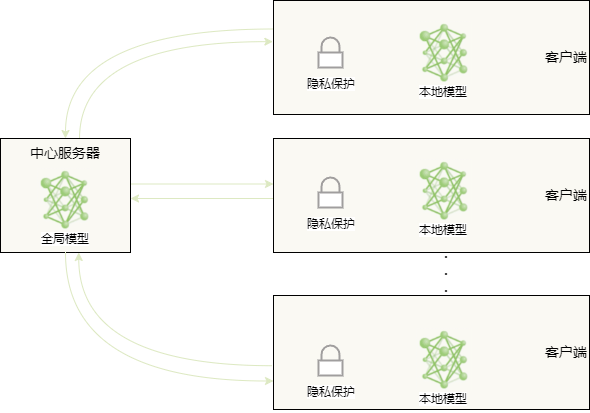
\includegraphics[width=10cm]{chapters/imgs/FedArch3} % 插入图像,设置图像的宽度为10cm
	\bicaption[\xiaosi 联邦学习系统架构]
	{\wuhao 联邦学习系统架构}
	{\wuhao Federated learning system architecture}
	\label{FedArch}
\end{figure}
\vspace{-0.35cm}

在整个工作流程中,中心服务器首先会初始化全局模型并将模型参数广播给所有客户端。各客户端在接收到这些参数后,利用本地数据进行训练,然后将更新后的本地模型(不包含原始数据)发送回中心服务器。聚合器再对所有客户端的模型参数进行加权平均等聚合操作,以生成新的全局模型。这个过程反复进行,直至模型收敛或达到预先设定的最大迭代次数。

联邦学习与分布式学习的主要区别在于对本地数据集特性所作假设不同\textsuperscript{\cite{konevcny2015federated}}。分布式学习旨在利用并行计算能力,通常假设每个本地数据集均为独立同分布(i.i.d.)且规模大致相同。而联邦学习则不做这些假设,它设计用于处理异构数据,数据集的规模可能存在显著差异。此外,联邦学习中的客户端往往较为不可靠,因其通常依赖于如 Wi-Fi 等较不稳定的通信方式,并运行在电池供电的设备(如智能手机或物联网设备)上,因此面临更高的失败或中途退出风险。相比之下,分布式学习通常依赖于数据中心内的节点,这些节点具备强大的计算能力,并通过高速网络互联\textsuperscript{\cite{kairouz2021advances}}。联邦学习的核心思想是在不共享数据的情况下训练模型,仅交换模型参数。

\subsection{联邦学习分类}
联邦学习可根据特征空间和样本空间的重叠情况,主要划分为横向联邦学习(Horizontal Federated Learning)、纵向联邦学习(Vertical Federated Learning)以及联邦迁移学习(Federated Transfer Learning)\textsuperscript{\cite{yang2019federated,li2020federated}},如图 \ref{FedClass} 所示。这种划分方式能够帮助研究人员与工程实践者在不同场景下选择适宜的联邦学习方案,从而更高效地利用分布式数据进行模型训练。

\vspace{-0.1cm}
\begin{figure}[!h]
	\centering
	\subfigure[]{
		\label{FedClassA}
		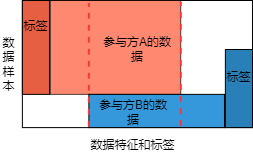
\includegraphics[width=0.3\textwidth]{chapters/imgs/FedClassA}}
	\hspace{0.01\textwidth}
	\subfigure[]{
		\label{FedClassB}
		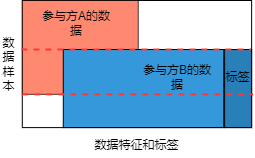
\includegraphics[width=0.3\textwidth]{chapters/imgs/FedClassB}}
	\hspace{0.01\textwidth}
	\subfigure[]{
		\label{FedClassC}
		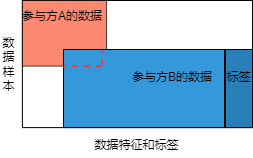
\includegraphics[width=0.3\textwidth]{chapters/imgs/FedClassC}}	
	\bicaption[\xiaosi \songti 联邦学习分类]
	{\centering \wuhao 联邦学习分类。(a) 横向联邦学习;(b) 纵向联邦学习;(c) 迁移联邦学习}
	{\centering \wuhao Federated Learning Classification. (a) Horizontal Federated Learning; (b) Vertical Federated Learning; (c) Transfer Federated Learning}	
	\label{FedClass}
\end{figure}
\vspace{-0.35cm}
在横向联邦学习(HFL)中,各数据拥有方在特征空间上较为相似,但用户或样本并不重叠\textsuperscript{\cite{yang2019federated,liu2019communication}},如图 \ref{FedClass}\subref{FedClassA} 所示。举例来说,若多家银行都想联合训练一个信用风险评估模型,但它们各自的用户群体并无明显重叠,且每家银行都有较为类似的特征字段(如年龄、职业、收入等),这种场景便适合采用横向联邦学习。通过让各银行保留本地数据,仅传递模型参数或梯度进行聚合,既能提升模型的泛化能力,又在最大程度上保护了用户隐私。

与之相对,纵向联邦学习(VFL)则适用于样本空间高度重叠,但特征集差异较大的场景\textsuperscript{\cite{liu2020secure,chen2020vafl}},如图 \ref{FedClass}\subref{FedClassB} 所示。例如,某些银行与电商平台在用户群体上可能有很大交集,却掌握了不同维度的用户信息:银行侧有用户财务信用数据,电商侧则有用户消费行为数据。在这种情形下,联合建模可以充分利用双方不同来源的特征信息,从而获得更全面、更准确的刻画。当各方在训练过程中只需对对齐后的公共用户进行联合梯度更新时,无需共享原始数据,依然能够保证个人隐私与数据安全。

第三种形式是联邦迁移学习(FTL),其特点在于样本空间与特征空间均不完全重叠\textsuperscript{\cite{yang2019federated,chen2020vafl}},如图 \ref{FedClass}\subref{FedClassC} 所示。在部分数据量较少或者特征不足的场景里,可以通过迁移学习的方法来补充数据或特征不足的问题。此时,不同组织或机构拥有的用户群体与特征集合可能仅存在少量重叠,但依然可通过联邦迁移学习的思想,将部分预训练模型的知识进行迁移,从而提升任务的性能或模型的泛化能力。这种方法特别适用于小样本或垂域知识不足的情景,有效地拓展了联邦学习在更多应用场景下的可行性。

综上所述,横向联邦学习、纵向联邦学习及联邦迁移学习分别应对了特征空间或样本空间上的不同重叠情况。它们在数据类型、业务场景和技术实现上各有侧重,却都遵循了联邦学习的核心理念:在不直接交换数据的前提下,实现多方协作与知识共享。这种多元化的联邦学习形式为不同行业和应用需求提供了灵活的选择,也在隐私保护和跨域协作方面展现出巨大的潜力。
\section{半监督学习}
\subsection{半监督学习概念}
在实际任务中,有标注数据往往十分稀缺,且标注过程需要投入大量的人力与时间成本。然而,大量的未标注数据通常容易获取,如果能够加以有效利用,便能显著提升模型的学习性能\textsuperscript{\cite{2015Semi}}。

半监督学习的核心思想在于同时利用少量标注数据与大量未标注数据进行联合训练,从而提升模型的泛化能力\textsuperscript{\cite{van2020survey}}。通过对未标注数据的“挖掘”或“自学习”,半监督学习有效弥补了标注样本不足所带来的数据缺陷\textsuperscript{\cite{van2020survey}}。

半监督学习通常建立在以下三个基本假设之上:首先,平滑性假设(Smoothness Assumption)认为在特征空间距离较近的样本,其标签也应相近;其次,聚类假设(Cluster Assumption)指出同一簇中的样本倾向于具有相同的标签;最后,低密度分隔假设(Low-density Separation Assumption)认为不同类别被低密度区域所分隔。

与监督学习相比,半监督学习更加强调对未标注数据的有效利用;而与无监督学习相比,半监督学习则依靠少量标注样本对模型进行指导,使模型能够在庞大的未标注数据中学习到更具区分度的特征\textsuperscript{\cite{van2020survey}}。
\subsection{半监督学习方法}

(2) 伪标签生成方法

该方法基于自训练(Self-training)假设\textsuperscript{\cite{lee2013pseudo}},通过为未标记数据生成伪标签来实现半监督学习,并将这些伪标签作为额外的训练数据。未标记数据对应的损失项通常可以表示为:
\begin{equation}\label{eq:2-1}
	L_u = \frac{1}{n} \sum_{i=1}^{n} \sum_{j=1}^{K} R \Bigl( y_i^{j}, \, p(x_i \mid \theta) \Bigr)
\end{equation}
其中,$ p(x_i \mid \theta) = \mathrm{softmax}\bigl(f(\theta, x_i)\bigr) $ 为模型 $ f(\theta) $ 在样本 $ x_i $ 上的预测概率分布,而 $ y_i^{j} $ 则指生成的伪标签,可以是一热编码或概率向量。为了实现熵最小化,通常采用一热编码的形式,使模型在预测时更加自信,从而将决策边界放置在低密度区域。当使用软标签时,为了达到类似的熵最小化效果,往往会对伪标签进行锐化处理,例如采用 0-1 阈值化:
\begin{equation}\label{eq:2-2}
	y_i^{j} = \mathrm{argmax}\Bigl(p(\theta', x_i)\Bigr)
\end{equation}
即直接以当前模型的预测作为伪标签。

在上述表达式中,$ R(\cdot, \cdot) $ 表示用于度量差异的距离函数,常用的包括均方误差(MSE)或交叉熵等\textsuperscript{\cite{van2020survey}}。为了进一步保留那些置信度较高的伪标签样本,可对公式 \eqref{eq:2-1} 进行更深层次的优化,通过引入一个筛选函数 $\mathrm{Filter}(\cdot)$ 来实现:
\begin{equation}\label{eq:2-3}
	L_u = \frac{1}{n} \sum_{i=1}^{n} \sum_{j=1}^{K} 
	\mathrm{Filter} \Bigl( R \bigl( y_i^{j},\, p(x_i \mid \theta) \bigr) \Bigr)
\end{equation}
使得模型仅聚焦于高可信度的伪标签样本。

此外,为了构建总的目标函数,常将带标签数据上的监督损失与未标记数据上的伪标签损失结合,得到:
\begin{equation}\label{eq:2-4}
	L = L_s + \alpha \, L_u
\end{equation}
其中,$ \alpha $ 用于平衡两部分损失,既可视为一个固定超参数,也可以随训练迭代而动态调整(如 $\alpha = \alpha(t)$)。通过对 $ L $ 的梯度进行反向传播并更新模型参数,模型会在每次迭代中不断重新预测未标记数据的伪标签,从而持续提升模型对未标记数据的刻画能力,直至收敛或满足预设的终止条件。


(2) PU(Positive and Unlabeled)学习

正例与未标注(Positive and Unlabeled,PU)学习是一种有效的半监督学习策略,旨在仅依赖少量确证的正例样本与大量未标注数据来构建分类模型,而无需明确的负例样本\textsuperscript{\cite{elkan2008learning,mordelet2013bagging}}。在传统的二分类场景中,研究人员通常需要完整且平衡的正负例数据集以训练模型。然而,随着数据规模的指数级增长,人工标注的成本与难度显著上升,大量真实世界数据缺乏可靠标记。为应对这一挑战,PU 学习通过将未知标签样本纳入训练过程,减少对全面标注的依赖,同时利用少量的正例样本来学习准确的决策边界。

近年来,PU 学习方法在多个领域均展现出卓越潜力。与传统方法相比,PU 学习无需显式负例,也能有效定位负类分布或异常模式,并对类别不平衡问题进行修正\textsuperscript{\cite{elkan2008learning}}。此外,PU 学习对大规模未标注数据的需求大幅降低了标注成本,尤其适合工业监测与异常检测等场景:在此类应用中,异常事件极为稀少,未标注数据往往代表了正常状态,因此仅使用少量正例便可使算法逐步“发掘”潜在负类特征,从而显著提升分类器的稳健性。

一种直接而高效的方法是将已标记的正例样本视为正类,而将未标注样本简单地视为负类进行训练\textsuperscript{\cite{elkan2008learning}}。尽管这一策略在理论上可能显得过于简化,但已有研究表明它仍能取得令人满意的实验效果。根据 Elkan 与 Noto\textsuperscript{\cite{elkan2008learning}} 的理论,当满足一定假设(例如正例样本是随机抽取的标注数据)时,仅基于正例与未标注数据训练得到的分类器,其输出分数与使用完整正负例数据训练的分类器之间存在正比关系。因此,在对样本进行排序或评估其成为正例的可能性时,这种简单方法的排名性能可与使用完整标注数据训练的模型相媲美。

进一步地,Mordelet 与 Vert\textsuperscript{\cite{mordelet2013bagging}} 提出了针对PU学习的改进袋装法(PU Bagging)。该方法首先在构建训练集时采用自助采样策略,即保留所有正例样本,并从未标注数据集中有放回地随机抽取一部分样本作为伪负例;随后利用“正例+伪负例”的自助样本训练分类器,并将训练好的分类器应用于未参与本轮自助抽样的未标注样本,记录这些袋外样本的预测得分;最后通过重复上述自助采样与训练过程,每个未标注样本将获得多个袋外预测分数,并以这些分数的平均值作为最终预测结果。

实验表明,当正例样本数量稀少或者未标注数据中负类比例本就较低时,PU Bagging方法往往表现优异,甚至能够超越某些更复杂的PU学习算法。此外,由于PU Bagging方法在处理大规模未标注数据时具备较高的计算效率,更适用于实际工业场景中的在线或分布式训练需求。

目前,多数 PU 学习算法通常可以归纳为 “两步法”,其主要步骤为首先进行可靠负样本识别,从未标注数据中筛选出高置信度的负例子集。尽管其规模可能较小,但标签质量较高,为后续训练提供基准。接着进行迭代分类器训练,将已知正例与前一步识别的可靠负例合并训练初始分类器,然后将该分类器应用到剩余的未标注数据。这个过程通常会进行多次迭代,随着更多可靠负例被标识并加入训练集,分类器的决策边界不断得到精炼,直至满足停止准则或取得收敛。

虽然两步法在机制上与 Shubham Jain 的 “伪标签” 策略相似,但其针对 PU 问题进行了专门设计,通过动态更新和扩充可靠负集来逐步提升分类器性能。相比于一般的半监督学习,两步法在 PU 场景下更强调对未知类别分布的主动探索,因而能在缺乏负例注释的环境中持续改进模型的判别能力。
\section{表格数据生成}
表格数据生成(Tabular Data Generation)是指通过一定的算法或模型,基于现有真实数据或先验知识,合成出具有与真实数据相似统计分布和特征的虚拟表格数据。随着大数据与隐私保护需求的不断增长,表格数据生成技术在医疗、金融、电商、社交媒体等领域具有越来越重要的应用价值。该技术不仅可以用于数据扩增(Data Augmentation)和算法测试,还能够在保证隐私安全的前提下,为数据分析和机器学习模型提供更多的训练样本\textsuperscript{\cite{li2021survey}}。

表格数据生成技术的核心目标在于在保持数据特征分布与关联关系的同时,最大程度地提升所生成数据的真实性与多样性,其典型生成过程需要综合考虑多个方面。生成数据需与真实数据在数值特征和类别特征上保持相似的分布特征,以避免重要特征的偏差或缺失,同时在多列或多特征维度的表格数据中捕捉并保留不同字段间复杂的相关性\textsuperscript{\cite{zhang2020tab}}。此外,生成过程还需兼顾隐私保护,既要避免暴露个体敏感信息,又要保证数据的可用性和真实性,而为了满足大规模数据需求,生成技术的效率和可扩展性也成为重要的考量指标。

当前,针对表格数据的生成方法主要分为基于统计模型和基于深度生成模型两大类,前者通过参数化或非参数化的统计分布对真实数据进行建模,后者则更多依赖神经网络,尤其是生成对抗网络(GAN)和变分自动编码器(VAE)等框架来生成高维度和多样化的数据\textsuperscript{\cite{brown2019differential}}。基于统计模型的方法通过对单变量分布及变量间相关关系建模,能够生成近似真实分布的数据,实现简单且具备一定可解释性,但在数据相关性复杂或维度较高时容易出现失配。而近年来,GAN 和 VAE 等深度生成模型在图像、文本等领域取得显著成果后,也逐渐应用于表格数据生成。通过生成器与判别器间的对抗训练,这类方法能捕捉多维特征关系并生成高保真合成数据,然而通常需要大量样本训练,且在超参数选择与模型可解释性方面仍面临较大挑战。

\section{本章小结}
本章系统介绍了联邦半监督学习样本生成方法的核心理论与技术,为后续算法设计和实验分析奠定了基础。针对分布式环境下的数据隐私和标记数据稀缺问题,本章分别从联邦学习、半监督学习和表格数据生成三个方面展开讨论。

首先,回顾了联邦学习通过分布式协作实现数据隐私保护与模型优化的基本思想,具体分析了横向联邦、纵向联邦和联邦迁移学习在异构数据处理与样本对齐中的优势与挑战。其次,阐述了半监督学习利用少量标记数据与大量未标记数据进行学习的基本范式,重点介绍了伪标签生成和正未标记(Positive and Unlabeled, PU)学习方法,为联邦学习框架下的半监督技术提供支持。最后,讨论了基于统计模型和深度生成模型的表格数据生成技术,强调其在数据扩充和隐私保护方面的潜力,为解决联邦学习中的样本不足与特征缺失问题提供了思路。

综上所述,本章明确了联邦学习、半监督学习和表格数据生成技术在解决数据隐私和性能优化问题中的协同作用,为后续提出的 VFPU 和 VFPU-M-Syn 等方法奠定了理论和技术基础。下一章将进一步探讨基于多方联邦的半监督学习方法,分析其在未标记数据缺失场景中的应用与表现。
